\documentclass{article}

\usepackage{amsmath, amsfonts}
\usepackage{float}
\usepackage{geometry}
\usepackage{graphicx}
\usepackage[table]{xcolor}
\usepackage{tikz}
\usetikzlibrary{matrix}
\usepackage{algorithm}
\usepackage{algpseudocode}
\usepackage{multicol}

\newgeometry{margin=1.25in}

\newcommand{\set}[1]{\lbrace #1 \rbrace}
\newcommand{\boundedBy}[1]{\mathcal{O} \left ( #1 \right )}
\newcommand{\expected}[1]{\mathbb{E} \left ( #1 \right )}
\newcommand{\exprv}[1]{\text{Exp} \left( #1 \right )}
\newcommand{\uniformrv}[2]{\mathcal{U} \left( #1, #2 \right )}
\newcommand{\FuncCall}[2]{\textsc{#1} \left ( #2 \right )}

\begin{document}

\author{Garrett Lewellen}
\title{A Greedy Approxmation Algorithm for the Linear Assignment Problem}

\maketitle

\section{Introduction}

The Linear Assignment Problem (LAP) is concerned with uniquely matching an equal number of workers to tasks, $n$, such that the overall cost of the pairings is minimized. A polynomial time algorithm was developed in the late fifties by \cite{kuhn1955hungarian}, and further refined by \cite{munkres1957algorithms}, called the Hungarian method. Named so after the work of Hungarian mathematicans K{\"o}nig and Egerv{\'a}ry whose theorems in the 1930s form the basis for the method. While the Hungarian Method can solve LAP instances in $\boundedBy{n^3}$ time, we wish to find faster algorithms even if it means sacraficing optimality in the process. Here we examine a greedy $\alpha$-approximation algorithm with $\boundedBy{n^2 \log n}$ runtime in terms of its approximation factor and compare it empircally to the Hungarian method.

\section{Linear Assignment Problem}

\begin{equation}
\begin{aligned}
	C_n = \min & \sum_{i=1}^{n} \sum_{j=1}^{n} M_{i,j} x_{i,j} \\
	s.t. & \sum_{i=1}^{n} x_{i,j} = 1, \quad j = 1, \ldots, n \\
	& \sum_{j=1}^{n} x_{i,j} = 1, \quad i = 1, \dots, n
	\label{eqn:lap}
\end{aligned}
\end{equation}

The LAP is given by the above linear program where $M \in \mathbb{Z}_{+}^{n \times n}$ cost matrix, and $x \in \lbrace 0,1 \rbrace^{n \times n}$ assignment matrix. This is equivalent to finding a perfect matching in a weighted bipartite graph. A minimal cost may have several possible assignments, but we are only interested in finding just one. It is assumed that no one worker can do all jobs more efficiently by themself than the distributing work across all workers. Likewise, if the costs are thought of durations, then the minimum cost is the minimum sequential rather than parallel time taken to complete the tasks.

From a practical point of view, we may relax the integral constraint on $M$ and allow all positive real-valued costs. For instances where there are more jobs than workers, and vice versa, dummy entries valued greater than the existing maximum may be added. Minimizing the cost is the default objective, but the maximum cost can be found by finding the optimal assignment for $M^{\prime}_{i,j} = M_{max} - M_{i,j}$, then finding the cost relative to $M$. 

\section{Algorithms}

\paragraph{Brute Force}

Rather than using the mathematical programming or graph theoretic representation of the problem, we can instead view the problem as finding the assignment that minimizes the cost out of all possible assignments:

\begin{equation}
	\pi^{*} = \underset{\pi \in \Pi_n}{\arg\min} \sum_{i=1}^{n} M_{i, \pi_i}
\end{equation}

There are $n!$ such assignments which can be produced using an iterative version of Heap's algorithm \cite{heap1963permutations} in $\boundedBy{n!}$ time assuming one does differential scoring (opposed to calculating the score for each permutation which would result in an $\boundedBy{n^2 (n-1)!}$ algorithm.)

\paragraph{Random}

The random algorithm selects a permutation $\pi \in \Pi_n$ uniformly from the set of all possible assignment permutations in $\boundedBy{n}$ time using the Fisher-Yates shuffle \cite{durstenfeld1964algorithm}. This obviously does not produce an optimal or near-optimal solution, but serves as a strawman to compare other results.

\paragraph{Greedy}

The greedy heuristic continues to cover the row and column of the smallest uncovered entry in the cost matrix until all entries are covered. The resulting set of entries then consitutes the assignment of workers to jobs. An inefficient $\boundedBy{n^3}$ algorithm can be used to find the smallest entry every iteration, or a more efficient result of $\boundedBy{n^2 \log n}$ can be obtained through the use of a sorted, array indexed hybrid mesh and queue. Let \texttt{QNode} represent a tuple consisting of row, column, and value; the previous entry in the matrix $\le$ this value, and the next entry in this matrix $\ge$ this value; and the \texttt{QNode}s (left, above, right, below) that are adjacent to this node.

\begin{algorithm}
\begin{algorithmic}
\Procedure{Greedy}{$M$} \Comment{$n \times n$ cost matrix}
\State $A[i] \gets \bot$ for $i = 0 \ldots n - 1$ \Comment{Assignment $A[$job$] = $ worker}
\State $Q[i] \gets$ \texttt{QNode} for $i = 0 \ldots n^2 - 1$
\State $\FuncCall{LinkMesh}{Q}$ \Comment{Adjacent node left, above, right, below properties}
\State $\FuncCall{Sort}{Q}$ \Comment{Sort in ascending order by node value}
\State $\FuncCall{LinkQueue}{Q}$ \Comment{Adjacent node previous and next properties}
\State $Q_{min} \gets Q[0]$
\While{$Q_{min} \neq nil$}
	\State $A[ Q_{min} \rightarrow row ] \gets Q_{min} \rightarrow col$
	\State $Q_{min} \gets \FuncCall{DeleteNode}{Q, Q_{min}}$ \Comment{Deletes row and col of $Q_{min}$}
\EndWhile
\State \textbf{return} $A$
\EndProcedure
\end{algorithmic}
\caption{A greedy algorithm for the LAP.}
\label{alg:greedy}
\end{algorithm}

\paragraph{} Allocating and linking for assignment is $\boundedBy{n}$; mesh $\boundedBy{n^2}$; queue $\boundedBy{2n^2\log n + n^2}$. Therefore, initialization requires $\boundedBy{n^2 \log n}$ time. The body of the loop requires a constant time assignment of worker to job, and $\boundedBy{2k - 1}$ time to remove the row and column from a $k \times k$ matrix using a modified depth first search. Thus the loop itself accounts for $\boundedBy{n^2}$ time. The resulting time complexity is therefore $\boundedBy{n^2 \log n} \square$.

\begin{equation*}
\quad
\begin{pmatrix}
62 & 31 & 79 & \fbox{6} & 21 & 37 \\
45 & 27 & 23 & 66 & \fbox{9} & 17 \\
83 & 59 & 25 & 38 & 63 & \fbox{25} \\
\fbox{1} & 37 & 53 & 100 & 80 & 51 \\
69 & \fbox{72} & 74 & 32 & 82 & 31 \\
34 & 95 & \fbox{61} & 64 & 100 & 82 \\
\end{pmatrix}
\quad
\begin{pmatrix}
62 & 31 & 79 & \fbox{6} & 21 & 37 \\
45 & 27 & 23 & 66 & \fbox{9} & 17 \\
83 & 59 & \fbox{25} & 38 & 63 & 25 \\
\fbox{1} & 37 & 53 & 100 & 80 & 51 \\
69 & 72 & 74 & 32 & 82 & \fbox{31} \\
34 & \fbox{95} & 61 & 64 & 100 & 82 \\
\end{pmatrix}
\end{equation*}

\paragraph{} Breaking ties for the minimum uncovered value can result in different costs. This drawback is shown in the above example were choosing $25$ at $(3,6)$ yields a minimum cost of $174$, where as the one at $(3, 3)$ gives a minimum cost of $167$. The next progression in the design of the greedy algorithm would be to try all minimum positions and keep the top $k$ performing paths.

\paragraph{Hungarian} The general idea behind the Kuhn-Munkres algorithm is that if we are given an initial assignment, we can make further assignments and potentially retask workers until all workers have been tasked with a job. The high level sketch of the algorithm starts with an initial assignment. While we have jobs that are unassigned, we look for qualified workers, ie, the zero entries. If a worker is already assigned to a job, but is also qualified for another, then we prime the alternative and continue to the next qualified worker, but if that is the only job the worker is qualified for, then we'd like to reassign any other worker already tasked to that job. This leads to a natural ripple effect represented by an alternating path of starred and primed entries. In Munkres' paper \cite{munkres1957algorithms} "starred" zero's represent assignments of workers to jobs, and "primed" zero's are alternative assignments. By flipping the bits of the path, we retask workers to their alternative tasks while ensuring the assignment continues to be minimal by construction. After assigning as many workers as we have to, we then deduct the lowest cost to create a new qualified worker. Thus, every iteration we are guaranteed to make positive progress towards our goal of finding an optimal assignment. This scheme results requires in the worst case $\boundedBy{n^3}$ time to complete.

\begin{algorithm}
\begin{algorithmic}
\Procedure{HungarianMethod}{$M$} \Comment{$n \times n$ cost matrix}
\State $M_{i,j} \gets M_{i,j} - \min_j M_{i,j}$ for $ i = 0 \ldots n - 1$
\State $M_{i,j} \gets M_{i,j} - \min_i M_{i,j}$ for $ j = 0 \ldots n - 1$
\State Star the first uncovered zero in row $i$, cover the corresponding column $j$ for $ i = 0 \ldots n - 1$

\While{ All columns not covered }
	\While{ Uncovered zeros }
		\State Prime the current uncovered zero
		\If{ There's a starred zero in this row }
			\State Uncover the starred zero's column and cover the row
		\Else
			\State Find an alternating augmented path from the primed zero
			\State Unstar the starred zeros on the path and star the primed zeros on the path
			\State Remove all the prime markings and cover all stared zeros
			\State \textbf{break}
		\EndIf
	\EndWhile

	\If {Found path}
		\State \textbf{continue}
	\EndIf

	\State $M^* = \min M_{i,j}$ over all uncovered $i, j$
	\State $M_{i,j} = M_{i,j} - M^*$ for all uncovered columns $j$
	\State $M_{i,j} = M_{i,j} + M^*$ for all covered rows $i$
\EndWhile

\State \textbf{return} Starred zeros \Comment{These are all the assignments}
\EndProcedure
\end{algorithmic}
\caption{The Hungarian method for the LAP.}
\label{alg:hungarian}
\end{algorithm}

To further illustrate the algorithm, consider the following example where starred entries are denoted by red, and primed entries by green:

\resizebox{\linewidth}{!}{
	\begin{tabular}{p{2.25in}p{2.25in}p{2.25in}}
		\noindent 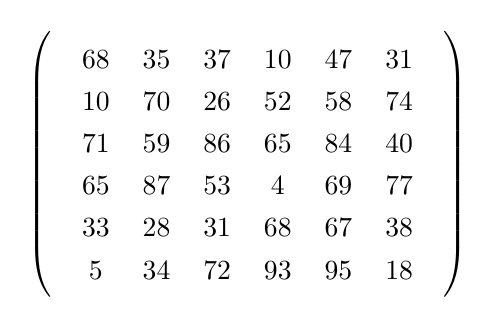
\begin{tikzpicture}
\matrix (M)[matrix of math nodes, column sep=-\pgflinewidth, row sep=-\pgflinewidth, left delimiter={(}, right delimiter={)}, nodes={anchor=center, align=center, minimum height=0.55cm, text width=0.55cm}] {
68 & 35 & 37 & 10 & 47 & 31 \\
10 & 70 & 26 & 52 & 58 & 74 \\
71 & 59 & 86 & 65 & 84 & 40 \\
65 & 87 & 53 & 4 & 69 & 77 \\
33 & 28 & 31 & 68 & 67 & 38 \\
5 & 34 & 72 & 93 & 95 & 18 \\
};
\end{tikzpicture}

&

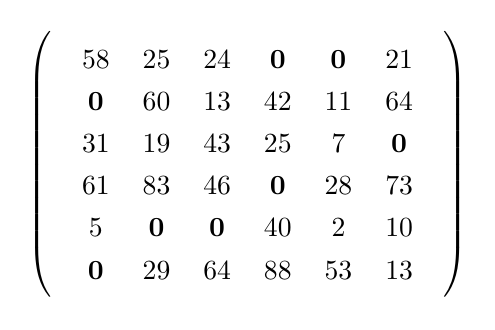
\begin{tikzpicture}
\matrix (M)[matrix of math nodes, column sep=-\pgflinewidth, row sep=-\pgflinewidth, left delimiter={(}, right delimiter={)}, nodes={anchor=center, align=center, minimum height=0.55cm, text width=0.55cm}] {
58 & 25 & 24 & \textbf{0} & \textbf{0} & 21 \\
\textbf{0} & 60 & 13 & 42 & 11 & 64 \\
31 & 19 & 43 & 25 & 7 & \textbf{0} \\
61 & 83 & 46 & \textbf{0} & 28 & 73 \\
5 & \textbf{0} & \textbf{0} & 40 & 2 & 10 \\
\textbf{0} & 29 & 64 & 88 & 53 & 13 \\
};
\end{tikzpicture}

&

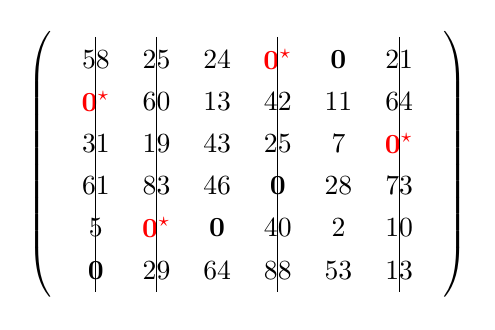
\begin{tikzpicture}
\matrix (M)[matrix of math nodes, column sep=-\pgflinewidth, row sep=-\pgflinewidth, left delimiter={(}, right delimiter={)}, nodes={anchor=center, align=center, minimum height=0.55cm, text width=0.55cm}] {
58 & 25 & 24 & \textcolor{red}{\textbf{0}^{\star}} & \textbf{0} & 21 \\
\textcolor{red}{\textbf{0}^{\star}} & 60 & 13 & 42 & 11 & 64 \\
31 & 19 & 43 & 25 & 7 & \textcolor{red}{\textbf{0}^{\star}} \\
61 & 83 & 46 & \textbf{0} & 28 & 73 \\
5 & \textcolor{red}{\textbf{0}^{\star}} & \textbf{0} & 40 & 2 & 10 \\
\textbf{0} & 29 & 64 & 88 & 53 & 13 \\
};
\draw[black] (M-1-1.north) -- (M-6-1.south);
\draw[black] (M-1-2.north) -- (M-6-2.south);
\draw[black] (M-1-4.north) -- (M-6-4.south);
\draw[black] (M-1-6.north) -- (M-6-6.south);
\end{tikzpicture}

\\

Input cost matrix

&

Deduct row, then resulting column minimums

&

Cover columns of starred entries

\\

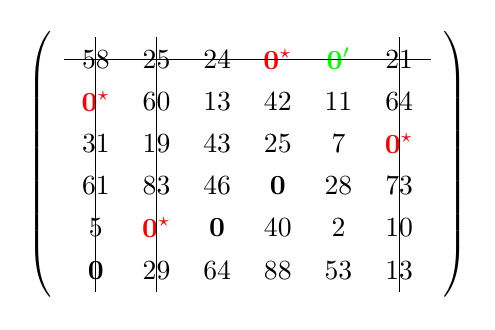
\begin{tikzpicture}
\matrix (M)[matrix of math nodes, column sep=-\pgflinewidth, row sep=-\pgflinewidth, left delimiter={(}, right delimiter={)}, nodes={anchor=center, align=center, minimum height=0.55cm, text width=0.55cm}] {
58 & 25 & 24 & \textcolor{red}{\textbf{0}^{\star}} & \textcolor{green}{\textbf{0}^{\prime}} & 21 \\
\textcolor{red}{\textbf{0}^{\star}} & 60 & 13 & 42 & 11 & 64 \\
31 & 19 & 43 & 25 & 7 & \textcolor{red}{\textbf{0}^{\star}} \\
61 & 83 & 46 & \textbf{0} & 28 & 73 \\
5 & \textcolor{red}{\textbf{0}^{\star}} & \textbf{0} & 40 & 2 & 10 \\
\textbf{0} & 29 & 64 & 88 & 53 & 13 \\
};
\draw[black] (M-1-1.west) -- (M-1-6.east);
\draw[black] (M-1-1.north) -- (M-6-1.south);
\draw[black] (M-1-2.north) -- (M-6-2.south);
\draw[black] (M-1-6.north) -- (M-6-6.south);
\end{tikzpicture}

&

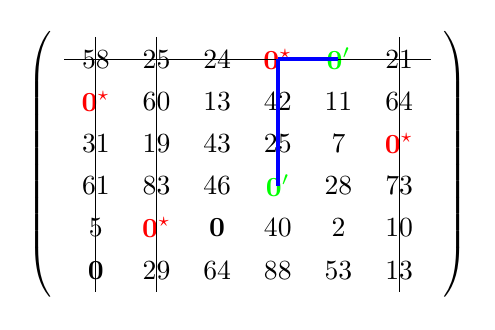
\begin{tikzpicture}
\matrix (M)[matrix of math nodes, column sep=-\pgflinewidth, row sep=-\pgflinewidth, left delimiter={(}, right delimiter={)}, nodes={anchor=center, align=center, minimum height=0.55cm, text width=0.55cm}] {
58 & 25 & 24 & \textcolor{red}{\textbf{0}^{\star}} & \textcolor{green}{\textbf{0}^{\prime}} & 21 \\
\textcolor{red}{\textbf{0}^{\star}} & 60 & 13 & 42 & 11 & 64 \\
31 & 19 & 43 & 25 & 7 & \textcolor{red}{\textbf{0}^{\star}} \\
61 & 83 & 46 & \textcolor{green}{\textbf{0}^{\prime}} & 28 & 73 \\
5 & \textcolor{red}{\textbf{0}^{\star}} & \textbf{0} & 40 & 2 & 10 \\
\textbf{0} & 29 & 64 & 88 & 53 & 13 \\
};
\draw[black] (M-1-1.west) -- (M-1-6.east);
\draw[black] (M-1-1.north) -- (M-6-1.south);
\draw[black] (M-1-2.north) -- (M-6-2.south);
\draw[black] (M-1-6.north) -- (M-6-6.south);
\draw[blue, ultra thick] (M-4-4.center) -- (M-1-4.center);
\draw[blue, ultra thick] (M-1-4.center) -- (M-1-5.center);
\end{tikzpicture}

&

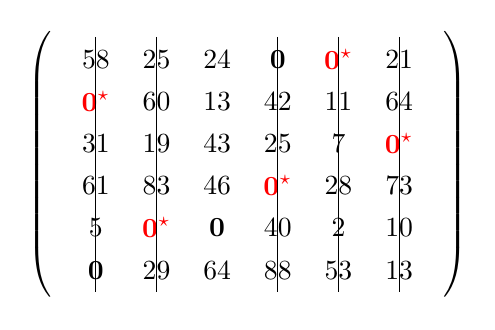
\begin{tikzpicture}
\matrix (M)[matrix of math nodes, column sep=-\pgflinewidth, row sep=-\pgflinewidth, left delimiter={(}, right delimiter={)}, nodes={anchor=center, align=center, minimum height=0.55cm, text width=0.55cm}] {
58 & 25 & 24 & \textbf{0} & \textcolor{red}{\textbf{0}^{\star}} & 21 \\
\textcolor{red}{\textbf{0}^{\star}} & 60 & 13 & 42 & 11 & 64 \\
31 & 19 & 43 & 25 & 7 & \textcolor{red}{\textbf{0}^{\star}} \\
61 & 83 & 46 & \textcolor{red}{\textbf{0}^{\star}} & 28 & 73 \\
5 & \textcolor{red}{\textbf{0}^{\star}} & \textbf{0} & 40 & 2 & 10 \\
\textbf{0} & 29 & 64 & 88 & 53 & 13 \\
};
\draw[black] (M-1-1.north) -- (M-6-1.south);
\draw[black] (M-1-2.north) -- (M-6-2.south);
\draw[black] (M-1-4.north) -- (M-6-4.south);
\draw[black] (M-1-5.north) -- (M-6-5.south);
\draw[black] (M-1-6.north) -- (M-6-6.south);
\end{tikzpicture}

\\

Starred zero at $(1, 4)$, prime $(1, 5)$

&

No starred zero in row $4$, prime $(4, 4)$ and find augmented path

&

Unstar starred entries and star prime entries along path

\\

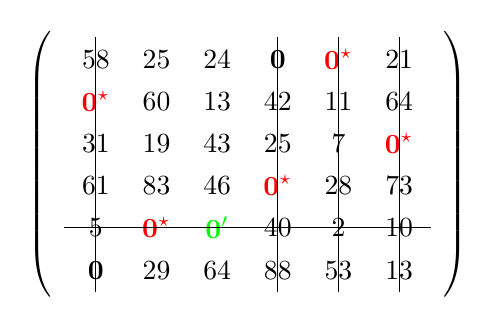
\begin{tikzpicture}
\matrix (M)[matrix of math nodes, column sep=-\pgflinewidth, row sep=-\pgflinewidth, left delimiter={(}, right delimiter={)}, nodes={anchor=center, align=center, minimum height=0.55cm, text width=0.55cm}] {
58 & 25 & 24 & \textbf{0} & \textcolor{red}{\textbf{0}^{\star}} & 21 \\
\textcolor{red}{\textbf{0}^{\star}} & 60 & 13 & 42 & 11 & 64 \\
31 & 19 & 43 & 25 & 7 & \textcolor{red}{\textbf{0}^{\star}} \\
61 & 83 & 46 & \textcolor{red}{\textbf{0}^{\star}} & 28 & 73 \\
5 & \textcolor{red}{\textbf{0}^{\star}} & \textcolor{green}{\textbf{0}^{\prime}} & 40 & 2 & 10 \\
\textbf{0} & 29 & 64 & 88 & 53 & 13 \\
};
\draw[black] (M-5-1.west) -- (M-5-6.east);
\draw[black] (M-1-1.north) -- (M-6-1.south);
\draw[black] (M-1-4.north) -- (M-6-4.south);
\draw[black] (M-1-5.north) -- (M-6-5.south);
\draw[black] (M-1-6.north) -- (M-6-6.south);
\end{tikzpicture}

&

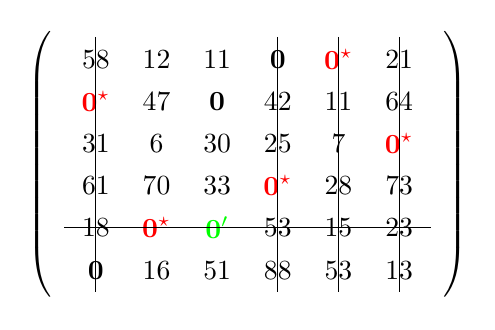
\begin{tikzpicture}
\matrix (M)[matrix of math nodes, column sep=-\pgflinewidth, row sep=-\pgflinewidth, left delimiter={(}, right delimiter={)}, nodes={anchor=center, align=center, minimum height=0.55cm, text width=0.55cm}] {
58 & 12 & 11 & \textbf{0} & \textcolor{red}{\textbf{0}^{\star}} & 21 \\
\textcolor{red}{\textbf{0}^{\star}} & 47 & \textbf{0} & 42 & 11 & 64 \\
31 & 6 & 30 & 25 & 7 & \textcolor{red}{\textbf{0}^{\star}} \\
61 & 70 & 33 & \textcolor{red}{\textbf{0}^{\star}} & 28 & 73 \\
18 & \textcolor{red}{\textbf{0}^{\star}} & \textcolor{green}{\textbf{0}^{\prime}} & 53 & 15 & 23 \\
\textbf{0} & 16 & 51 & 88 & 53 & 13 \\
};
\draw[black] (M-5-1.west) -- (M-5-6.east);
\draw[black] (M-1-1.north) -- (M-6-1.south);
\draw[black] (M-1-4.north) -- (M-6-4.south);
\draw[black] (M-1-5.north) -- (M-6-5.south);
\draw[black] (M-1-6.north) -- (M-6-6.south);
\end{tikzpicture}

&

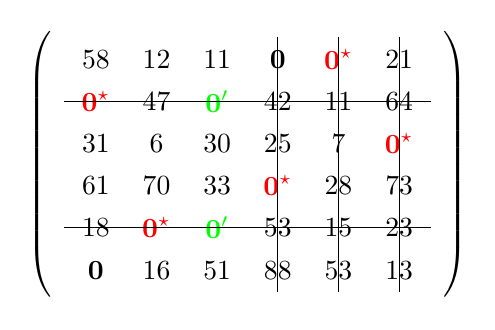
\begin{tikzpicture}
\matrix (M)[matrix of math nodes, column sep=-\pgflinewidth, row sep=-\pgflinewidth, left delimiter={(}, right delimiter={)}, nodes={anchor=center, align=center, minimum height=0.55cm, text width=0.55cm}] {
58 & 12 & 11 & \textbf{0} & \textcolor{red}{\textbf{0}^{\star}} & 21 \\
\textcolor{red}{\textbf{0}^{\star}} & 47 & \textcolor{green}{\textbf{0}^{\prime}} & 42 & 11 & 64 \\
31 & 6 & 30 & 25 & 7 & \textcolor{red}{\textbf{0}^{\star}} \\
61 & 70 & 33 & \textcolor{red}{\textbf{0}^{\star}} & 28 & 73 \\
18 & \textcolor{red}{\textbf{0}^{\star}} & \textcolor{green}{\textbf{0}^{\prime}} & 53 & 15 & 23 \\
\textbf{0} & 16 & 51 & 88 & 53 & 13 \\
};
\draw[black] (M-2-1.west) -- (M-2-6.east);
\draw[black] (M-5-1.west) -- (M-5-6.east);
\draw[black] (M-1-4.north) -- (M-6-4.south);
\draw[black] (M-1-5.north) -- (M-6-5.south);
\draw[black] (M-1-6.north) -- (M-6-6.south);
\end{tikzpicture}

\\

Starred zero at $(5, 1)$, prime $(5, 3)$

&

No uncovered zeros, deduct uncovered minimum and it to double covered entries

&

Starred zero at $(2, 1)$, prime $(2, 3)$

\\

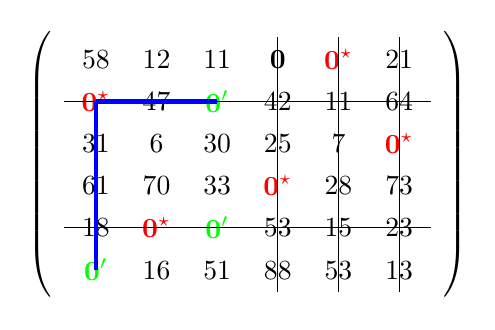
\begin{tikzpicture}
\matrix (M)[matrix of math nodes, column sep=-\pgflinewidth, row sep=-\pgflinewidth, left delimiter={(}, right delimiter={)}, nodes={anchor=center, align=center, minimum height=0.55cm, text width=0.55cm}] {
58 & 12 & 11 & \textbf{0} & \textcolor{red}{\textbf{0}^{\star}} & 21 \\
\textcolor{red}{\textbf{0}^{\star}} & 47 & \textcolor{green}{\textbf{0}^{\prime}} & 42 & 11 & 64 \\
31 & 6 & 30 & 25 & 7 & \textcolor{red}{\textbf{0}^{\star}} \\
61 & 70 & 33 & \textcolor{red}{\textbf{0}^{\star}} & 28 & 73 \\
18 & \textcolor{red}{\textbf{0}^{\star}} & \textcolor{green}{\textbf{0}^{\prime}} & 53 & 15 & 23 \\
\textcolor{green}{\textbf{0}^{\prime}} & 16 & 51 & 88 & 53 & 13 \\
};
\draw[black] (M-2-1.west) -- (M-2-6.east);
\draw[black] (M-5-1.west) -- (M-5-6.east);
\draw[black] (M-1-4.north) -- (M-6-4.south);
\draw[black] (M-1-5.north) -- (M-6-5.south);
\draw[black] (M-1-6.north) -- (M-6-6.south);
\draw[blue, ultra thick] (M-6-1.center) -- (M-2-1.center);
\draw[blue, ultra thick] (M-2-1.center) -- (M-2-3.center);
\end{tikzpicture}

&

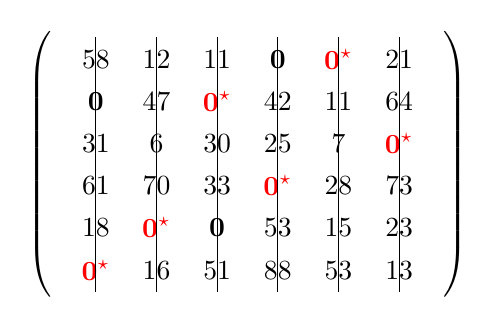
\begin{tikzpicture}
\matrix (M)[matrix of math nodes, column sep=-\pgflinewidth, row sep=-\pgflinewidth, left delimiter={(}, right delimiter={)}, nodes={anchor=center, align=center, minimum height=0.55cm, text width=0.55cm}] {
58 & 12 & 11 & \textbf{0} & \textcolor{red}{\textbf{0}^{\star}} & 21 \\
\textbf{0} & 47 & \textcolor{red}{\textbf{0}^{\star}} & 42 & 11 & 64 \\
31 & 6 & 30 & 25 & 7 & \textcolor{red}{\textbf{0}^{\star}} \\
61 & 70 & 33 & \textcolor{red}{\textbf{0}^{\star}} & 28 & 73 \\
18 & \textcolor{red}{\textbf{0}^{\star}} & \textbf{0} & 53 & 15 & 23 \\
\textcolor{red}{\textbf{0}^{\star}} & 16 & 51 & 88 & 53 & 13 \\
};
\draw[black] (M-1-1.north) -- (M-6-1.south);
\draw[black] (M-1-2.north) -- (M-6-2.south);
\draw[black] (M-1-3.north) -- (M-6-3.south);
\draw[black] (M-1-4.north) -- (M-6-4.south);
\draw[black] (M-1-5.north) -- (M-6-5.south);
\draw[black] (M-1-6.north) -- (M-6-6.south);
\end{tikzpicture}

&

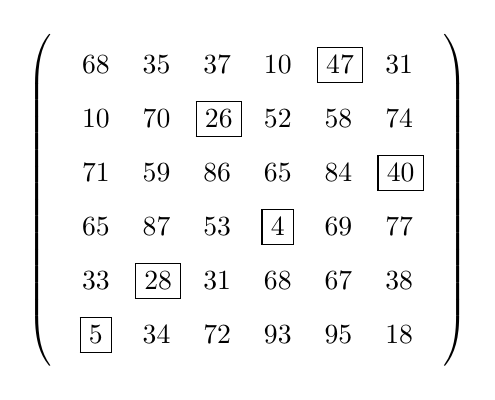
\begin{tikzpicture}
\matrix (M)[matrix of math nodes, column sep=-\pgflinewidth, row sep=-\pgflinewidth, left delimiter={(}, right delimiter={)}, nodes={anchor=center, align=center, minimum height=0.55cm, text width=0.55cm}] {
68 & 35 & 37 & 10 & \fbox{47} & 31 \\
10 & 70 & \fbox{26} & 52 & 58 & 74 \\
71 & 59 & 86 & 65 & 84 & \fbox{40} \\
65 & 87 & 53 & \fbox{4} & 69 & 77 \\
33 & \fbox{28} & 31 & 68 & 67 & 38 \\
\fbox{5} & 34 & 72 & 93 & 95 & 18 \\
};
\end{tikzpicture}
\\


No starred zero in row $6$, prime $(6, 1)$ and find augmented path

&

Unstar starred entries and star prime entries along path

&

Output cost of 150

	\end{tabular}
}

\section{Analysis}

The prevailing convention in the literature is to look at the approximation factor, $\alpha$, to determine how close the results of an approximation algorithm are to optimal. Here this ratio is the expected minimum cost assignment of the algorithm under test to the same quantity given by the expected minimum assignment cost. Let $M_{i,j} \sim \exprv{1}$ be an $n \times n$ a standard exponential random cost matrix. We resort to the exponential distribution for its ease of analyis and prominence in related literature. Cf. the works of \cite{kurtzberg1962approximation}, \cite{michael1990probability} for analysis based on $M_{i,j} \sim \mathcal{U}(0,1)$.

\paragraph{Exponential Distribution Properties}

Let $X \sim \exprv{\lambda}$ have cumulative distribution function $F_X(x) = 1 - \exp{\left(-\lambda x\right)}$ and expectation $\expected{X} = \lambda^{-}$. Define the order statistic $X_{1:n} = \min \lbrace X_{1}, \ldots, X_{n} \rbrace $ to be the minimum of $n$ draws from $\exprv{\lambda}$. $X_{1:n} \sim \exprv{n \lambda}$ \cite{balakrishnan2000handbook} with expectation $\expected{X_{1:n}} = \left(n \lambda\right)^-$. Let $Y_n = \sum_{i = 1}^{n} X_i \sim \text{Gamma}(n, \lambda)$ with expectation $\expected{Y_n} = n \lambda^{-}$.

\paragraph{Expected Minimum Cost}

The expected minimum assignment cost for $M$ is given by \cite{aldous2001zeta}:

\begin{equation}
	\expected{C_n} = \sum_{k = 1}^{n} \frac{1}{k^2} = H_{n}^{(2)}
\end{equation}

Which is the generalized Harmonic Number of order two and converges to $\zeta(2) = \pi^2/6$.

\paragraph{Greedy}

The minimum value of an $n \times n$ matrix is given by the order statistic $M^{1:n^2} = \min \set{ M_{1,1} \ldots M_{n, n} }$ with expectation $\expected{ M_{1:n^2} } = n^{-2}$. The expected value of the minimum cost assignment is not just $\sum_{i=0}^{n-1} (n-i)^2$ because the expectation doesn't take into account the previous iteration's minimum value. To accomplish this we make use of the memoryless property of the exponential distribution to observe that the expected difference in minimums betweens iterations is the expected minimum value given by $M_{i:k^2}$. If we add up all these differences we get the expected minimum value of the k'th iteration; summing all these expectations then yields the expected minimum cost assignment:

\begin{equation}
	\expected{C_n} = \sum_{i=0}^{n-1} \sum_{j=0}^{i} \frac{1}{(n - j)^2} = \sum_{j=0}^{n-1} \frac{(n-j)}{(n-j)^2} = \sum_{j=0}^{n-1} \frac{1}{n-j} = H_n
\end{equation}

This is the Harmonic Number of order one which does not converge. The resulting approximation factor is:

\begin{equation}
	\alpha_n = \frac{H_n}{H_n^{(2)}}
\end{equation}

\paragraph{Random}

The random algorithm will simply select an assignment permutation, so we are just adding up $n$ $\exprv{1}$ distributed random variables leading to an expected cost of: 

\begin{equation}
	\expected{C_n} = \sum_{i=1}^n \expected{ M_{i, \pi_i} } = n
\end{equation}

And approximation factor:

\begin{equation}
	\alpha_n = \frac{n}{H_n^{(2)}}
\end{equation}

\section{Evaluation}

To illustrate the preceeding results, Figure \ref{fig:approximationFactor} shows the approximation factor for the greedy algorithm implementations against the derived approximation factor. The simulated results are based on 120 $n times n$ standard exponentially distributed matrices for $1 \le n \le 1000$. 

\begin{multicols}{2}
\begin{figure}[H]
	\centering
	\resizebox{\linewidth}{!}{\input{obj/approximationFactor.tex}}
	\caption{Greedy analytical and empirical approximation factor with 95\% confidence interval.}
	\label{fig:approximationFactor}
\end{figure}

\columnbreak

\begin{figure}[H]
	\centering
	\resizebox{\linewidth}{!}{\input{obj/runtime.tex}}
	\caption{Elapsed wall time with 95\% confidence interval.}
	\label{fig:runtime}
\end{figure}
\end{multicols}

Using the same conventions for the approximation factor, Figure \ref{fig:runtime} illustrates the runtime characteristics of the algorithms. Results obtained from source code compiled with -O3 flags and ran on a Xeon E3-1245 v5 3.4 Ghz system with 32 GBs of 2133Mhz DDR4 RAM. Ignoring constant factors, the algorithms coincide with the theoretical expectations.

\section{Summary}

\begin{table}[H]
	\centering
	\begin{tabular}{l|c|c|c|c}
& Brute & Random & Greedy & Hungarian \\
\hline
Complexity & $\boundedBy{n!}$ & $\boundedBy{n}$ & $\boundedBy{n^2 \log n}$ & $\boundedBy{n^3}$ \\
$\alpha_n$ & 1 & $\frac{n}{H_n^{(2)}}$ & $\frac{H_n}{H_n^{(2)}}$ & 1
	\end{tabular}
	\caption{Merits of each approach}
\end{table}

For exact solutions, the brute method is suitable for instances involving a handful of workers, but the Hungarian method is suitable for all other instances. Approximate solutions can be provided by the greedy algorithm with logarithmic degeneracy while providing a linear factor improvement over the Hungarian method.

\bibliographystyle{acm}
\bibliography{doc/references}

\end{document}
